% DPF 09 talk on strangeness in nucleon

\documentclass[10pt]{beamer}
\usepackage{amsmath}
\usepackage{mathtools}
\usefonttheme{professionalfonts} % using non standard fonts for beamer
\usefonttheme{serif} % default family is serif
%\documentclass[12pt]{beamerthemeSam.sty}
\usepackage{epsf}
%\usepackage{pstricks}
%\usepackage[orientation=portrait,size=A4]{beamerposter}
\geometry{paperwidth=160mm,paperheight=120mm}
\usepackage{tikz}

\newcommand{\shrug}[1][]{%
\begin{tikzpicture}[baseline,x=0.8\ht\strutbox,y=0.8\ht\strutbox,line width=0.125ex,#1]
\def\arm{(-2.5,0.95) to (-2,0.95) (-1.9,1) to (-1.5,0) (-1.35,0) to (-0.8,0)};
\draw \arm;
\draw[xscale=-1] \arm;
\def\headpart{(0.6,0) arc[start angle=-40, end angle=40,x radius=0.6,y radius=0.8]};
\draw \headpart;
\draw[xscale=-1] \headpart;
\def\eye{(-0.075,0.15) .. controls (0.02,0) .. (0.075,-0.15)};
\draw[shift={(-0.3,0.8)}] \eye;
\draw[shift={(0,0.85)}] \eye;
% draw mouth
\draw (-0.1,0.2) to [out=15,in=-100] (0.4,0.95); 
\end{tikzpicture}}

%DT favorite definitions
\def\LL{\left\langle}	% left angle bracket
\def\RR{\right\rangle}	% right angle bracket
\def\LP{\left(}		% left parenthesis
\def\RP{\right)}	% right parenthesis
\def\LB{\left\{}	% left curly bracket
\def\RB{\right\}}	% right curly bracket
\def\PAR#1#2{ {{\partial #1}\over{\partial #2}} }
\def\PARTWO#1#2{ {{\partial^2 #1}\over{\partial #2}^2} }
\def\PARTWOMIX#1#2#3{ {{\partial^2 #1}\over{\partial #2 \partial #3}} }

\def\rightpartial{{\overrightarrow\partial}}
\def\leftpartial{{\overleftarrow\partial}}
\def\diffpartial{\buildrel\leftrightarrow\over\partial}

\def\BI{\begin{itemize}}
\def\EI{\end{itemize}}
\def\BE{\begin{displaymath}}
\def\EE{\end{displaymath}}
\def\BEA{\begin{eqnarray*}}
\def\EEA{\end{eqnarray*}}
\def\BNEA{\begin{eqnarray}}
\def\ENEA{\end{eqnarray}}
\def\EL{\nonumber\\}


\newcommand{\map}[1]{\frame{\frametitle{\textbf{Course map}}
\centerline{\includegraphics[height=0.86\paperheight]{../../map/#1.png}}}}
\newcommand{\wmap}[1]{\frame{\frametitle{\textbf{Course map}}
\centerline{\includegraphics[width=0.96\paperwidth]{../../map/#1.png}}}}

\newcommand{\etal}{{\it et al.}}
\newcommand{\gbeta}{6/g^2}
\newcommand{\la}[1]{\label{#1}}
\newcommand{\ie}{{\em i.e.\ }}
\newcommand{\eg}{{\em e.\,g.\ }}
\newcommand{\cf}{cf.\ }
\newcommand{\etc}{etc.\ }
\newcommand{\atantwo}{{\rm atan2}}
\newcommand{\Tr}{{\rm Tr}}
\newcommand{\dt}{\Delta t}
\newcommand{\op}{{\cal O}}
\newcommand{\msbar}{{\overline{\rm MS}}}
\def\chpt{\raise0.4ex\hbox{$\chi$}PT}
\def\schpt{S\raise0.4ex\hbox{$\chi$}PT}
\def\MeV{{\rm Me\!V}}
\def\GeV{{\rm Ge\!V}}

%AB: my color definitions
%\definecolor{mygarnet}{rgb}{0.445,0.184,0.215}
%\definecolor{mygold}{rgb}{0.848,0.848,0.098}
%\definecolor{myg2g}{rgb}{0.647,0.316,0.157}
\definecolor{abtitlecolor}{rgb}{0.0,0.255,0.494}
\definecolor{absecondarycolor}{rgb}{0.0,0.416,0.804}
\definecolor{abprimarycolor}{rgb}{1.0,0.686,0.0}
\definecolor{Red}           {cmyk}{0,1,1,0}
\definecolor{Grey}           {cmyk}{.4,.4,.4,0}
\definecolor{Lg}           {cmyk}{.4,.4,.4,0}
\definecolor{Blue}          {cmyk}{1,1,0,0}
\definecolor{Green}         {cmyk}{1,0,1,0}
\definecolor{Brown}         {cmyk}{0,0.81,1,0.60}
\definecolor{Black}         {cmyk}{0,0,0,1}

\usetheme{Madrid}


%AB: redefinition of beamer colors
%\setbeamercolor{palette tertiary}{fg=white,bg=mygarnet}
%\setbeamercolor{palette secondary}{fg=white,bg=myg2g}
%\setbeamercolor{palette primary}{fg=black,bg=mygold}
\setbeamercolor{title}{fg=abtitlecolor}
\setbeamercolor{frametitle}{fg=abtitlecolor}
\setbeamercolor{palette tertiary}{fg=white,bg=abtitlecolor}
\setbeamercolor{palette secondary}{fg=white,bg=absecondarycolor}
\setbeamercolor{palette primary}{fg=black,bg=abprimarycolor}
\setbeamercolor{structure}{fg=abtitlecolor}

\setbeamerfont{section in toc}{series=\bfseries}

%AB: remove navigation icons
\beamertemplatenavigationsymbolsempty
\title[Angular momentum and moment of inertia]{
  \textbf {Angular momentum and moment of inertia}\\
%\centerline{}
%\centering
%\vspace{-0.0in}
%\includegraphics[width=0.3\textwidth]{propvalues_0093.pdf}
%\vspace{-0.3in}\\
%\label{intrograph}
}

\author[W. Freeman] {Physics 211\\Syracuse University, Physics 211 Spring 2016\\Walter Freeman}

\date{\today}

\begin{document}

\frame{\titlepage}

\frame{\frametitle{\textbf{Announcements}}
\large
Exam 2 is next Tuesday. Exam prep schedule:
\BI
\item{Today: office hours 3:30-5:30}
\item{Tomorrow: {\bf extra office hours 12-6}}
\item{Thursday: office hours 1:30-3:30}
\item{Friday: morning office hours 10-2, review session 1-4, location TBD}
\pause
\item{Saturday afternoon: review session in Stolkin, 4-7 PM}
\EI
}

\frame{\frametitle{\textbf{Computational project 2: recap}}
\BI
\large
\item{This project was substantially more detailed than the last one}
\item{If you didn't finish, you may finish up during my office hours this week: bring your laptop to the Clinic}
\item{... if you didn't skip recitation last week! (I will be checking...)}
\BI
\item{Excused absences are as always excused}
\EI
\EI
}

\frame{\frametitle{\textbf{Rotational motion}}
\large
Before, you learned that rotational kinematics worked the same way as translational kinematics:

\bigskip

    \large
\centerline{  \begin{tabular}{| c | c |}
    \hline
    Translation & Rotation \\
    \hline
    \hline
    \hline
    Position $x$ & Angle $\theta$ \\
    \hline
    Velocity $v$ & Angular velocity $\omega$ \\
    \hline
    Acceleration $a$ & Angular acceleration $\alpha$ \\
    \hline
    \hline
    $v(t) = v_0 + at$ & $\omega(t) = \omega_0 + \alpha t$ \\
    \hline
    $x(t) = x_0 + v_0 t + \frac{1}{2}at^2$ & $\theta(t) = \theta_0 + \omega_0 t + \frac{1}{2} \alpha t^2$ \\
    \hline
    $v_f^2 - v_0^2 = 2a \Delta x$ & $ \omega_f^2 - \omega_0^2 = 2 \alpha \Delta \theta$ \\
    \hline
  \end{tabular}
}

\pause

\bigskip

Since then, you've learned some other physical ideas relating to translational motion: {\color{Red} Newton's second law} and {\color{Red}conservation of momentum}.

\pause

\bigskip

... do they have rotational counterparts as well?}


\frame{\frametitle{\textbf{Rotational motion counterparts: just conceptual, for now}}
\begin{columns}
\column{0.5\textwidth}
\color{Blue}
\Large
\centerline{Translational motion}
\normalsize
\BI
\item{Forces make things accelerate}
\item{Mass resists that acceleration}
\item{$\vec F = m \vec a$}
\item{Moving objects have momentum}
\item{$\vec p = m \vec v$}
\item{Momentum conserved if there are no external forces}
\EI
\column{0.5\textwidth}
\color{Red}
\Large
\centerline{Rotational motion}
\normalsize
\BI
\item{{\color{Green}Torques $\tau$} give things an angular acceleration}
\item{{\color{Green}Moment of inertia $I$} resists that acceleration}
\item{$\tau = I \alpha$}
\item{Spinning objects have angular momentum $L$}
\item{$L = I \omega$}
\item{Angular momentum conserved if no external torques}
\EI
\end{columns}

\bigskip
\bigskip

\Large

$\rightarrow$ Torque: analogue of force

$\rightarrow$ Moment of inertia: analogue of mass

$\rightarrow$ $\tau = I \alpha$: equivalent to Newton's second law

$\rightarrow$ $L = I \omega = $ constant; analogue to conservation of momentum

}

\frame{\frametitle{\textbf{Today: conservation of momentum}}
\begin{columns}
\column{0.5\textwidth}
\color{Grey}
\Large
\centerline{Translational motion}
\normalsize
\BI
\color{Grey}
\item{Forces make things accelerate}
\item{Mass resists that acceleration}
\item{$\vec F = m \vec a$}
{\color{Red}
\item{Moving objects have momentum}
\item{$\vec p = m \vec v$}
\item{Momentum conserved if there are no external forces}}
\EI
\column{0.5\textwidth}
\color{Grey}
\Large
\centerline{Rotational motion}
\normalsize
\BI
\color{Grey}
\item{Torques $\tau$ give things an angular acceleration}
\item{Moment of inertia $I$ resists that acceleration}
\item{$\tau = I \alpha$}
{\color{Blue}
\item{Spinning objects have angular momentum $L$}
\item{$L = I \omega$}
\item{Angular momentum conserved if no external torques}}
\EI
\end{columns}

\bigskip
\bigskip

\Large
\color{Grey}
$\rightarrow$ Torque: analogue of force

$\rightarrow$ Moment of inertia: analogue of mass

$\rightarrow$ $\tau = I \alpha$: equivalent to Newton's second law
\color{Red}

$\rightarrow$ $L = I \omega = $ constant; analogue to conservation of momentum

}

\frame{\frametitle{\textbf{The plan for teaching you these things}}
\large
\BI
\item{The hardest part of this is learning to {\it calculate torque}, so we'll put that off until the end}
\item{Today (and on exam 2): angular momentum, only}
\item{We'll learn about rotational energy when we get to energy}
\item{Finally, we'll figure out the relation between torque to force and put it all together}
\EI
}


\frame{\frametitle{\textbf{Understanding moment of inertia}}

 \centerline{\Large The analogue of mass is called ``moment of inertia'' (letter $I$)}

  \BI
  \large
\item{More massive things are harder to turn, but that's only part of it}
\item{The mass {\it distribution} matters, too}
\item{The further the mass is from the center, the harder it will be to turn}
\item{The moment of inertia depends on the {\it average squared distance from the center}}
    \BI
  \item{\color{Lg}I state this without proof here; if you're interested in why, come see me!}
    \EI
  \EI

  \bigskip\pause

  \centerline{\Large $I=MR^2$}

\bigskip
\bigskip
\bigskip

  \centerline{\large ({\bf only} if all the mass is the same distance from the center)}
  \centerline{\large (our bike wheels and demo rods)}
}

\frame{\frametitle{\textbf{Moment of inertia, other things}}
  \centerline{\Large What about the moment of inertia of other objects?}
  \centerline{\large We need to average {$R^2$} over all of the mass in the object}

\medskip

  \centerline{\large Requires calculus in general; here are some common ones}
  \centerline{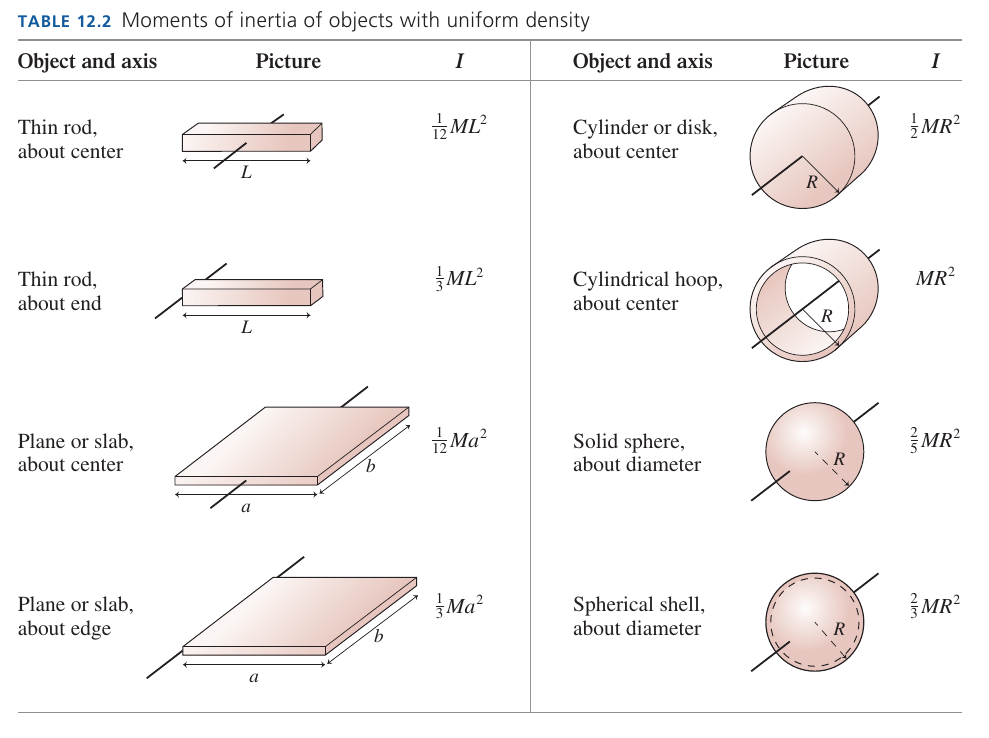
\includegraphics[width=0.7\textwidth]{moment-table.png}}
  }

\frame{\frametitle{\textbf{Conservation of angular momentum}}
\large
We saw that the conservation of momentum was valuable mostly in two sorts of situations:

\BI
\item{Collisions: two objects strike each other}
\item{Explosions: one object separates into two}
\EI

There is a third case for conservation of angular momentum:

\BI
\item{Collisions: two rotating things collide (a kid jumps on a rotating platform, HW problem 3)}
\item{Explosions: throwing a ball off-center (see our demo)}
\item{{\color{Red}A spinning object changes shape}}
\EI

\pause
\bigskip


This last happens because moment of inertia depends on {\it how the mass is distributed}, not just how much there is!

}

\frame{\frametitle{\textbf{Examples}}
\large

A person of mass $M=60 kg$ standing on a rotating platform holds two $m=2$ kg weights at arm's length $L$. If he spins at $\omega=1 s^{-1}$ and then pulls the weights
in toward his chest, what happens to his angular velocity?

}

\frame{\frametitle{\textbf{Examples}}
\large
A person of mass $M$ standing on a rotating platform is handed a bicycle wheel full of concrete. It has a mass of $m$ and is spinning at angular 
velocity $\omega$. If she turns it over, what happens to her?
}

\frame{\frametitle{\textbf{Examples}}
\large
A person of mass $M$ standing on a rotating platform catches a cannonball traveling at velocity $v$ a distance $r$ away from the center. 
What is his angular velocity after he catches it?

\pause

\bigskip
\bigskip
\bigskip

Need to know the angular momentum of the cannonball before the collision, but all we know is $v$. The trick: $\omega=v_T/r$, since the 
tangential velocity and $\omega$ are related.

For a point mass, remember $I=mr^2$.

\begin{align*}
L &= I\omega \\
L &= (mr^2) (v_T/r) \\
L &= m v_T r 
\end{align*}
}


\end{document}
